\documentclass[12pt,a4paper]{article}
\usepackage[utf8x]{inputenc}
\usepackage[english,hebrew]{babel}
\usepackage{graphicx}
\usepackage{verbatim}
\usepackage{url}

\usepackage{tikz}
\usetikzlibrary{external,positioning,through,calc,intersections,arrows.meta}
\tikzexternalize[prefix=tikz/]

\textwidth=15.5cm
\textheight=23cm
\topmargin=0pt
\headheight=0pt
\oddsidemargin=2em
\headsep=0pt
\renewcommand{\baselinestretch}{1.1}
\setlength{\parskip}{0.3\baselineskip plus 1pt minus 1pt}
\parindent=0pt

\newtheorem{exercise}{תרגיל}


\begin{document}
\thispagestyle{empty}

\selectlanguage{hebrew}

\begin{center}
\textbf{\Huge%
 איך לרבע את המעגל )בערך(
}

\bigskip

\bigskip

\textbf{\Large מוטי בן-ארי}

\bigskip

\textbf{\Large המחלקה להוראת המדעים}

\bigskip

\textbf{\Large מכון ויצמן למדע}

\bigskip

\url{http://www.weizmann.ac.il/sci-tea/benari/}
\end{center}

\bigskip
\bigskip

\begin{center}
\selectlanguage{english}
\copyright{}\  2017 by Moti Ben-Ari.

\end{center}

\selectlanguage{english}

{\small This work is licensed under the Creative Commons Attribution-ShareAlike 3.0 Unported License. To view a copy of this license, visit \url{http://creativecommons.org/licenses/by-sa/3.0/} or send a letter to Creative Commons, 444 Castro Street, Suite 900, Mountain View, California, 94041, USA.}

\bigskip

\begin{center}

\includegraphics[width=.2\textwidth]{../by-sa.png}
\end{center}

\selectlanguage{hebrew}

\newpage

\begin{center}
\textbf{\Large%
קירובים ל-%
$\pi$}
\end{center}

היוונים היו הראשונים שחקרו בנייה גיאומרטית עם סרגל ומחוגה. הם לא הצליחו לפתור שלוש בעיות: חלוקת זווית לשלושה, הכפלת קוביה )נתונה קוביה, בנה קוביה בנפח פי-שניים( וריבוע מעגל )נתון מעגל, בנה ריבוע עם אותו שטח(. במאה ה-91 הוכח שאין פתרונות לבעיות אלו.

באמצעות אלגברה ניתן להראות: אם נתונה קטע קו שאורכו
$1$,
המספרים )אורכי הקטעים( שניתן לבנות מהקטע הזה הם תוצאות של חישובים עם פעולות החשבון
$+,-,\times,\div,\surd$.
לא ניתן לבנות שורש שלישי, ולכן לא ניתן להכפיל קוביה, כי כדי להכפיל קוביה עם נפח 
$1$
חייבים לפתור את המשוואה
$x^3-2=0$,
ולבנות את האורך
$\sqrt[3]{2}$.
מאותה סיבה לא ניתן לחלק זווית שרירותית לשלושה, כי כדי לחלק 
$60^\circ$
חייבים לפתור את המשוואה מסדר שלוש
$8x^3-6x-1=0$.

חקר הבעיה של ריבוע המעגל היה איטי יותר ופתרון נמצא רק בשנת 2881. נתון מעגל יחידה ששטחו
$\pi r^2=\pi$,
יש לבנות ריבוע שהצלע שלו באורך
$\sqrt{\pi}$.
אבל
$\pi$
הוא מספר
\textbf{טרנסנדנטלי},
שמשמעותו היא שהמספר אינו פתרון של אף משוואה אלגבראית. ההוכחה מסובכת ביותר ומשתמשת במושגים מאנליזה ומספרים מרוכבים.

קיימים קירובים פשוטים מאוד ל-%
$\pi$,
למשל:
\[
\frac{355}{113}=3.14159292\,,
\]
שההפרש בינו לבין
$\pi\approx 3.14159265$
הוא רק 
$2.67\times 10^{-7}$.
רדיוס כדור הארץ הוא בערך
$6,378.1$
ק"מ. חישוב ההיקף עם
$355/113$
נותן תוצאה של
$40,074.78421$
ק"מ וחישוב עם
$\pi$
נותן תוצאה של
$40,074.78761$
ק"מ. ההפרש הוא פחות מ-%
$4$
מטר!

ניתן לבנות את המספר הרציונלי
$355/113$
על ידי הארכת קטע קו באורך אחד
$113$
פעמים,
הרחבת נוספת כדי לקבל קטע קו באורך 
$355$,
ובניית קטע קו שאורכו מתקבל מחילוק. מסמך זה מביא בנייה קצרה של קטע קו באורך
$355/113$
שפורסם על ידי
\textbf{רמנוג'ן}
\L{\textbf{Ramanujan}}
ב-\\
\L{\emph{Journal of the Indian Mathematical Society}, 1913, p. 138}.

נציג את הבנייה בשלבים ובכל שלב נציג תרגילים המבקשים שתשלים את החישובים. את התשובות ניתן למצוא בסוף המסמך, ביחד עם המאמר המקורי של רמנוג'ן.

רמנוג'ן
\L{(1887--1920)}
גדל בהודו במה שנקרא עכשיו מדינת
\L{Tamil Nadu}.
מהר מאוד הוא התקדם מעבר לרמה של בתי הספר והמכללות המקומיות. הוא שלח את עבודותיו למתמטיקאי האנגלי
\L{G.H. Hardy}
שהזמין אותו לאנגליה. רמנוג'ן הגיע בשנת 4191, וחזרתו להודו לא התאפשרה עד לסיום מלחמת העולם הראשונה. הוא סבל רבות ממזג האוויר הקר ומהאוכל הלא מוכר )כהינדי אדוק היה צמחוני(. זמן קצר לאחר שובו להודו נפטר בגיל 
$32$.
המתמטיקה שהגה רמנוג'ן נחקרת עד היום לאחר מאה שנים. ביאוגרפיה:

\L{Robert Kanigel. \emph{The Man Who Knew Infinity: A Life of the Genius Ramanujan}, 1991.}


\newpage

%%%%%%%%%%%%%%%%%      First

\begin{center}
\textbf{\Large שלב 1}
\end{center}

\begin{itemize}
\item
בנה מעגל יחידה עם מרכז
$O$
וקוטר
$PR$.
\item 
סמן
$H$
במחצית הקטע
$PO$,
וסמן
$T$
כשליש הקטע
$RO$.
\item
בנה אנך מ-%
$T$
שחותך את המעגל ב-%
$Q$.
\item 
בנה מיתר
$RS$
שאורכו שווה ל-%
$QT$.
\end{itemize}

\begin{center}
\selectlanguage{english}
\begin{tikzpicture}[scale=.9]
% Draw circle and horizontal diameter
\draw[name path=circle] (0,0)  coordinate (o) node[below] {$O$} circle[radius=5cm];
\draw (-5,0) coordinate (p) node[left] {$P$} -- (5,0) coordinate (r) node[right] {$R$};
\fill (o) circle (1pt);
\fill (p) circle (1pt);
\fill (r) circle (1pt);
\fill (-2.5,0) coordinate (h) node[below] {$H$} circle (1pt);
\fill (10/3,0) coordinate (t) node[below] {$T$} circle (1pt);
\path (p) -- node[above,xshift=12pt] {$1/2$} (h) -- node[above] {$1/2$} (o) -- node[above] {$2/3$} (t) -- node[above] {$1/3$} (r);
% Draw perpendicular TQ
\path[name path=tq] (t) -- +(0,5);
\path[name intersections={of=tq and circle,by=q}];
\draw (t) -- node[left] {$a$} (q) node[above] {$Q$};
\fill (q) circle (1pt);
% Draw chord RS
\path[name path=rcirc] (r) let \p1 = ($ (t) - (q) $) in circle ({veclen(\x1,\y1)});
\path[name intersections={of=rcirc and circle,by=s}];
\draw (r) -- node[left] {$a$} (s);
\fill (s) node[above right] {$S$} circle (1pt);
\draw (p) -- node[above] {$b$} (s);
\end{tikzpicture}
\end{center}

\begin{exercise}
בנה את האורך 
$TR=\displaystyle\frac{1}{3}$.
\end{exercise}

\begin{exercise}
חשב את אורכו של
$QT$.
\end{exercise}

\begin{exercise}
חשב את אורכו של
$PS$.
\end{exercise}

\begin{exercise}
בנה את המיתר
$QR=RS$.
\end{exercise}


\newpage

%%%%%%%%%%%%%%%%%      Second

\begin{center}
\textbf{\Large שלב 2}
\end{center}

\begin{itemize}
\item 
בנה קטעי קו
$NT$
ו-%
$OM$
מקביליים ל-%
$RS$.
\end{itemize}

\begin{center}
\selectlanguage{english}
\begin{tikzpicture}[scale=.9]
% Draw circle and horizontal diameter
\draw[name path=circle] (0,0)  coordinate (o) node[below] {$O$} circle[radius=5cm];
\draw (-5,0) coordinate (p) node[left] {$P$} -- (5,0) coordinate (r) node[right] {$R$};
\fill (o) circle (1pt);
\fill (p) circle (1pt);
\fill (r) circle (1pt);
\fill (-2.5,0) coordinate (h) node[below] {$H$} circle (1pt);
\fill (10/3,0) coordinate (t) node[below] {$T$} circle (1pt);
% Draw chord RS and line PS
\path[name path=tq] (t) -- +(0,5);
\path[name intersections={of=tq and circle,by=q}];
\path[name path=rcirc] (r) let \p1 = ($ (t) - (q) $) in circle ({veclen(\x1,\y1)});
\path[name intersections={of=rcirc and circle,by=s}];
\draw (r) -- node[left] {$a$} (s);
\fill (s) node[above right] {$S$} circle (1pt);
\draw[name path=ps] (p) -- node[above right,xshift=8pt,yshift=8pt] {$b$} (s);
% Draw TN
\path[name path=tn] (t) -- +($(s)-(r)$);
\path[name intersections={of=ps and tn,by=n}];
\draw (t) -- (n);
\fill (n) node[above] {$N$} circle (1pt);
% Draw OM
\path[name path=om] (o) -- +($(s)-(r)$);
\path[name intersections={of=ps and om,by=m}];
\draw (o) -- (m);
\fill (m) node[above left] {$M$} circle (1pt);
% Label PM and MN
\path (p) -- node[below,xshift=12pt,yshift=4pt] {$c$} (m);
\path (m) -- node[below,xshift=8pt,yshift=4pt] {$d$} (n);
\end{tikzpicture}
\end{center}

\begin{exercise}
חשב את אורכו של
$PM$.
\end{exercise}

\begin{exercise}
חשב את אורכו של
$MN$.
\end{exercise}

\newpage

%%%%%%%%%%%%%%%%%      Third

\begin{center}
\textbf{\Large שלב 3}
\end{center}


\begin{itemize}
\item
בנה את המיתר
$PK=PM$.
\item
בנה את המשיק
$PL=MN$.
\item 
חבר את הנקודות
$K,L,R$.
\end{itemize}

\begin{center}
\selectlanguage{english}
\begin{tikzpicture}[scale=.9]
% Draw circle and horizontal diameter
\draw[name path=circle] (0,0)  coordinate (o) node[below] {$O$} circle[radius=5cm];
\draw (-5,0) coordinate (p) node[left] {$P$} -- (5,0) coordinate (r) node[right] {$R$};
\fill (o) circle (1pt);
\fill (p) circle (1pt);
\fill (r) circle (1pt);
\fill (-2.5,0) coordinate (h) node[below] {$H$} circle (1pt);
\fill (10/3,0) coordinate (t) node[below] {$T$} circle (1pt);
% Draw chord RS and line PS
\path[name path=tq] (t) -- +(0,5);
\path[name intersections={of=tq and circle,by=q}];
\path[name path=rcirc] (r) let \p1 = ($ (t) - (q) $) in circle ({veclen(\x1,\y1)});
\path[name intersections={of=rcirc and circle,by=s}];
\draw (r) -- (s);
\fill (s) node[above right] {$S$} circle (1pt);
\draw[name path=ps] (p) -- (s);
% Draw TN
\path[name path=tn] (t) -- +($(s)-(r)$);
\path[name intersections={of=ps and tn,by=n}];
\draw (t) -- (n);
\fill (n) node[above] {$N$} circle (1pt);
% Draw OM
\path[name path=om] (o) -- +($(s)-(r)$);
\path[name intersections={of=ps and om,by=m}];
\draw (o) -- (m);
\fill (m) node[above left] {$M$} circle (1pt);
\path (p) -- node[below,xshift=12pt,yshift=4pt] {$c$} (m);
\path (m) -- node[below,xshift=8pt,yshift=4pt] {$d$} (n);
% Draw chord PK
\path[name path=pkcirc] (p) let \p1 = ($ (p) - (m) $) in circle ({veclen(\x1,\y1)});
\path[name intersections={of=pkcirc and circle,by={k1,k}}];
\draw (p) -- node[right,xshift=-2pt,yshift=10pt] {$c$} (k) node[below left] {$K$};
% Draw tangent PL
\draw let \p1 = ($ (m) - (n) $), \n1 = {veclen(\x1,\y1)} in (p) -- node[left] {$d$} (-5,-\n1) coordinate (l) node[left] {$L$};
% Connect L and K to R
\draw (r) -- node[above] {$f$} (l) -- (k) -- node[below right] {$e$} cycle;
\end{tikzpicture}
\end{center}

\begin{exercise}
מה ידוע על 
$\triangle PKR$?
חשב את אורכו של
$RK$.
\end{exercise}

\begin{exercise}
מה ידוע על
$\triangle LPR$?
חשב את אורכו של
$RL$.
\end{exercise}

\newpage

%%%%%%%%%%%%%%%%%      Fourth

\begin{center}
\textbf{\Large שלב 4}
\end{center}

\begin{itemize}
\item
סמן את הנקודה
$C$
כך ש-%
$RC=RH$.
\item 
בנה
$CD$
מקביל ל-%
$LK$.
\end{itemize}

\begin{center}
\selectlanguage{english}
\begin{tikzpicture}[scale=.9]
% Draw circle and horizontal diameter
\draw[name path=circle] (0,0)  coordinate (o) node[below] {$O$} circle[radius=5cm];
\draw (-5,0) coordinate (p) node[left] {$P$} -- (5,0) coordinate (r) node[right] {$R$};
\fill (o) circle (1pt);
\fill (p) circle (1pt);
\fill (r) circle (1pt);
\fill (-2.5,0) coordinate (h) node[below] {$H$} circle (1pt);
% Get values of PM and MN but don't draw
\coordinate (t) at (10/3,0);
\path[name path=tq] (t) -- +(0,5);
\path[name intersections={of=tq and circle,by=q}];
\path[name path=rcirc] (r) let \p1 = ($ (t) - (q) $) in circle ({veclen(\x1,\y1)});
\path[name intersections={of=rcirc and circle,by=s}];
\path[name path=ps] (p) -- (s);
\path[name path=tn] (t) -- +($(s)-(r)$);
\path[name intersections={of=ps and tn,by=n}];
\path[name path=om] (o) -- +($(s)-(r)$);
\path[name intersections={of=ps and om,by=m}];
% Draw chord PK
\path[name path=pkcirc] (p) let \p1 = ($ (p) - (m) $) in circle ({veclen(\x1,\y1)});
\path[name intersections={of=pkcirc and circle,by={k1,k}}];
\draw (p) -- (k) node[below left] {$K$};
% Draw tangent PL
\draw let \p1 = ($ (m) - (n) $), \n1 = {veclen(\x1,\y1)} in (p) -- (-5,-\n1) coordinate (l) node[left] {$L$};
% Connect L and K to R
\draw (r) -- node[above] {$f$} (l) -- (k) -- node[below right] {$e$} cycle;
% Find point C on RK
\coordinate (c) at ($(r)!7.5cm!(k)$);
\path (r) -- node[above, near end] {$g$} (c);
\fill (c) node[below] {$C$} circle (1pt);
% Draw CD
\path[name path=cd] (c) -- +($(l)-(k)$);
\path[name path=lr] (l) -- (r);
\path[name intersections={of=cd and lr,by=d}];
\draw (c) -- (d);
\fill (d) node[above,xshift=2pt] {$D$} circle (1pt);
\path (r) -- node[below,near end] {$h$} (d);
\end{tikzpicture}
\end{center}


\begin{exercise}
חשב את אורכו של
$RC$.
\end{exercise}

\begin{exercise}
חשב את אורכו של
$RD$.

\end{exercise}

\begin{exercise}
בנה ריבוע שאורך הצלע שלו הוא
$RD$.
\end{exercise}

\begin{exercise}
חשב את
$RD^2$
שהוא שטח הריבוע. חשב גם כשבר וגם כמספר עשרוני.
\end{exercise}

\newpage

%%%%%%%%%%%%%%%%%      Fifth

\begin{center}
\textbf{\Large סיכום}
\end{center}

להלן הבנייה בשלמותה כאשר כל האורכים מסומנים.

\bigskip

\begin{center}
\selectlanguage{english}
\begin{tikzpicture}[scale=1.2,align=left]
% Draw circle and horizontal diameter
\draw[name path=circle] (0,0)  coordinate (o) node[below] {$O$} circle[radius=5cm];
\draw (-5,0) coordinate (p) node[left] {$P$} -- (5,0) coordinate (r) node[right] {$R$};
\fill (o) circle (1pt);
\fill (p) circle (1pt);
\fill (r) circle (1pt);
\fill (-2.5,0) coordinate (h) node[below] {$H$} circle (1pt);
\fill (10/3,0) coordinate (t) node[below] {$T$} circle (1pt);
\path (p) -- node[above,xshift=10pt] {$1/2$} (h) -- node[above] {$1/2$} (o) -- node[above] {$2/3$} (t) -- node[above] {$1/3$} (r);
% Draw chord RS and line PS
\path[name path=tq] (t) -- +(0,5);
\path[name intersections={of=tq and circle,by=q}];
\path[name path=rcirc] (r) let \p1 = ($ (t) - (q) $) in circle ({veclen(\x1,\y1)});
\path[name intersections={of=rcirc and circle,by=s}];
\draw (r) -- node[right] {$\sqrt{5}/3$} (s);
\fill (s) node[above right] {$S$} circle (1pt);
\draw[name path=ps] (p) -- node[above right,yshift=16pt] {$\sqrt{31}/3$} (s);
% Draw TN
\path[name path=tn] (t) -- +($(s)-(r)$);
\path[name intersections={of=ps and tn,by=n}];
\draw (t) -- (n);
\fill (n) node[above] {$N$} circle (1pt);
% Draw OM
\path[name path=om] (o) -- +($(s)-(r)$);
\path[name intersections={of=ps and om,by=m}];
\draw (o) -- (m);
\fill (m) node[above left] {$M$} circle (1pt);
\path (p) -- node[below,xshift=32pt,yshift=12pt] {$\sqrt{31}/6$} (m);
\path (m) -- node[below,xshift=8pt,yshift=-6pt] {$\sqrt{31}/9$} (n);
% Draw chord PK
\draw (p) -- node[right,xshift=-2pt,yshift=10pt] {$\sqrt{31}/6$} +(-62.3:4.64) coordinate (k) node[below left] {$K$};
% Draw tangent PL
\draw let \p1 = ($ (m) - (n) $), \n1 = {veclen(\x1,\y1)} in (p) -- node[left] {$\sqrt{31}/9$} (-5,-\n1) coordinate (l) node[left] {$L$};
% Connect L and K to R
\draw (r) -- (l) -- (k) -- cycle;
% Find point C on RK
\coordinate (c) at ($(r)!7.5cm!(k)$);
\path (r) -- node[below,yshift=-16pt] {$RC=3/2$\\$RK=\sqrt{113}/6$} (c);
\fill (c) node[below] {$C$} circle (1pt);
% Draw CD
\path[name path=cd] (c) -- +($(l)-(k)$);
\path[name path=lr] (l) -- (r);
\path[name intersections={of=cd and lr,by=d}];
\draw (c) -- (d);
\fill (d) node[above,xshift=2pt] {$D$} circle (1pt);
\path (r) -- node[above,xshift=-40pt,yshift=-8pt] {$RD=\sqrt{355/113}$\\$RL=\sqrt{355}/9$} (d);
\end{tikzpicture}
\end{center}

\newpage

%%%%%%%%%%%%%%%%%%%%%%%%%%%%%%%  Answers

\begin{center}
\textbf{\Large תשובות לתרגילים}
\end{center}

\begin{enumerate}

\item
בנה
$\triangle ABC$
עם האורכים הרשומים ובנה 
$DE$
מקביל ל-%
$BC$. 
\begin{center}
\selectlanguage{english}
\begin{tikzpicture}
\draw (0,0) node[left] {$A$} -- (6,0) node[right] {$B$};
\path (0,0) -- node[below] {$1$} (2,0) coordinate (a1) node[below] {$D$} -- node[below] {$2$} (6,0);
\draw (6,0) -- node[right] {$1$} ++(100:2) coordinate (a2) node[above] {$C$};
\draw[name path=p1] (a2) -- (0,0);
\path[name path=p2] (2,0) -- ++(100:1);
\path[name intersections={of=p1 and p2,by=q}];
\draw (a1) -- node[right] {$n$} (q) node[above] {$E$};
\end{tikzpicture}
\end{center}
לפי משולשים דומים:
\[
\frac{n}{1} = \frac{1}{3}\,.
\]
\item
לפי משפרט פיתגורס:
$\triangle QOT$:
\[
QT = \sqrt{1^2-\left(\frac{2}{3}\right)^2}=\frac{\sqrt{5}}{3}\,.
\]

\item $\triangle PSR$
הוא משולש ישר זווית כי הוא כולא קוטר. לפי משפט פיתגורס:
\[
PS = \sqrt{2^2-\left(\frac{\sqrt{5}}{3}\right)^2}=\sqrt{4-\frac{5}{9}}=\frac{\sqrt{31}}{3}\,.
\]

\item
הצב את רגלי המחוגה על 
$QT$.
בנה מעגל עם מרכז 
$R$
ורדיוס זה.

\item
לפי המשולשים הדומים:
\[
\frac{PM}{PO}=\frac{PS}{PR},\;\;\;\frac{PM}{1}=\frac{\sqrt{31}/3}{2},\;\;\;PM=\frac{\sqrt{31}}{6}.
\]

\item
לפי המשולשים הדומים:
\[
\frac{PN}{PT}=\frac{PS}{PR},\;\;\;\frac{PN}{5/3}=\frac{\sqrt{31}/3}{2},\;\;\;PN=\frac{5\sqrt{31}}{18}\,.
\]
\[
MN=PN-PM = \sqrt{31}\left(\frac{5}{18}-\frac{1}{6}\right) = \frac{\sqrt{31}}{9}\,.
\]

\item $\triangle PKR$
הוא משולש ישר זווית כי הוא כולא קוטר. לפי משפט פיתגורוס:
\[
RK=\sqrt{2^2-\left(\frac{\sqrt{31}}{6}\right)^2} = \frac{\sqrt{113}}{6}\,.
\]

\item $\triangle PLR$
הוא משולש ישר זווית כי
$PL$
משיק. לפי משפט פיתגורס:
\[
RL=\sqrt{2^2+\left(\frac{\sqrt{31}}{9}\right)^2} = \frac{\sqrt{355}}{9}\,.
\]

\item $RC=RH=\displaystyle\frac{1}{3}+\frac{2}{3}+\frac{1}{2}=\frac{3}{2}$.

\item 
בגלל ש-%
$CD$
מקביל ל-%
$LK$,
לפי המשולשים הדומים:
\[
\frac{RD}{RC}=\frac{RL}{RK}\,,\;\;\;\frac{RD}{3/2}=\frac{\sqrt{355}/9}{\sqrt{113}/6}\,,\;\;\;RD=\sqrt{\frac{355}{113}}\,.
\]
\item
נתון קטע קו באורך
$RD$,
הארך אותו לקטע קו באורך
$3RD$.
בנה אנכים באורך
$RD$
מנקודות הקצה של הקטע האמצעי. חבר את קצות האנכים.
\begin{center}
\selectlanguage{english}
\begin{tikzpicture}
\draw (0,0) -- (6,0);
\foreach \i in {0,2,4,6}
  \fill (\i,0) circle (2pt);
\fill (2,2) circle (2pt);
\fill (4,2) circle (2pt);
\draw (2,2) -- (4,2);
\draw (2,0) -- (2,3);
\draw (4,0) -- (4,3);
\draw ([shift=(30:3.2cm)]0,0) arc (30:60:3.2cm);
\draw ([shift=(150:3.2cm)]4,0) arc (150:120:3.2cm);
\draw ([shift=(30:3.2cm)]2,0) arc (30:60:3.2cm);
\draw ([shift=(150:3.2cm)]6,0) arc (150:120:3.2cm);
\path (2,0) -- node[above] {$RD$} (4,0);
\end{tikzpicture}
\end{center}

\item \mbox{}
\[
\frac{355}{113}=3.14159292\,.
\]

\end{enumerate}

\selectlanguage{english}
\hspace*{-5em}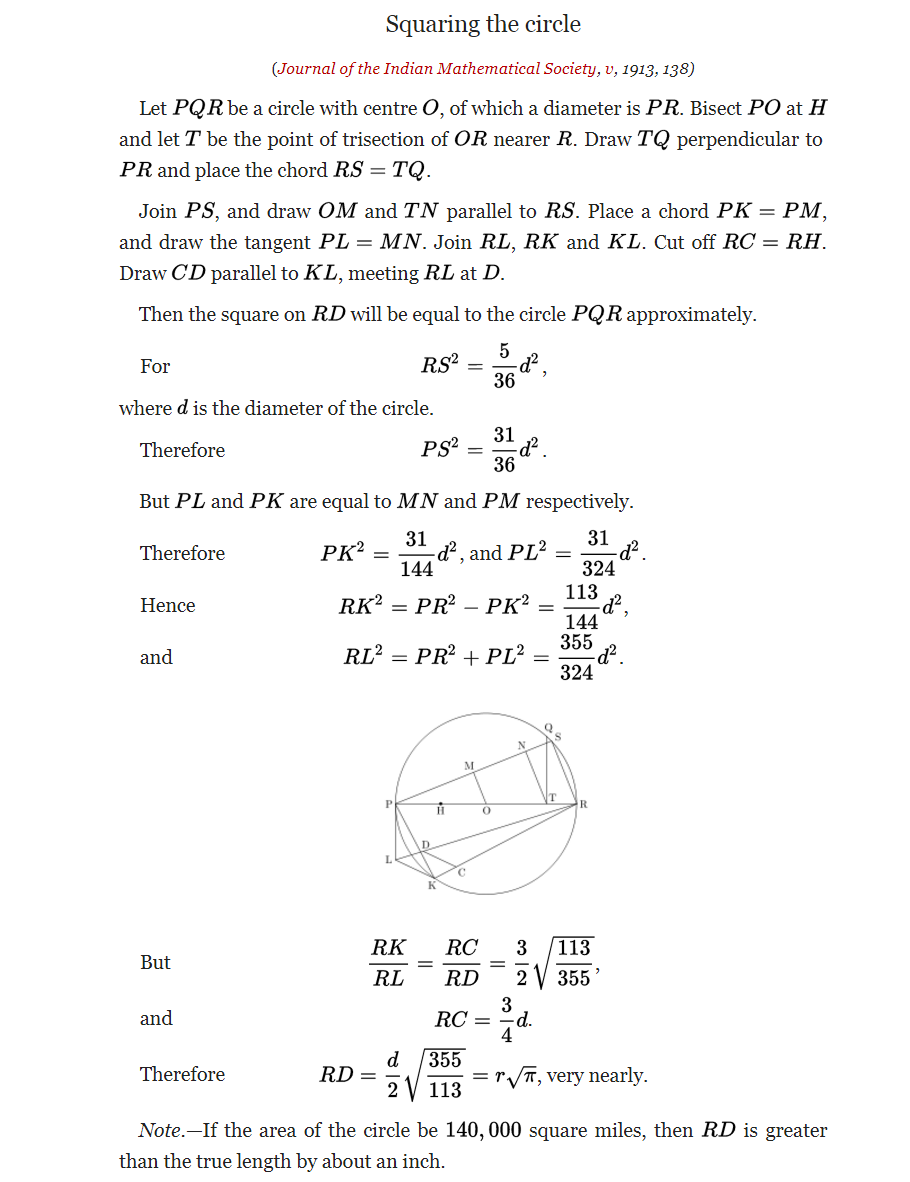
\includegraphics[width=1.2\textwidth]{ramanujan.png}

\end{document}
